%
% l2.tex -- L2 Räume 
%
% (c) 2019 Prof Dr Andreas Müller, Hochschule Rapperswil
%
\section{Der Hilbertraum $L^2$
\label{section:l2}}
\rhead{Der Hilbertraum $L^2$}

\subsection{Funktionenräume}
Wir bezeichnen mit $\mathbb C^X$ die Menge der Funktionen
$f\colon X\to \mathbb C$.
Sie wird auf natürliche Art zu einem Vektorraum, indem man die
Addition von Funktionen und die Multiplikation mit Skalaren
punktweise definiert.
Seien $f,g$ Funktionen auf $X$, dann definieren wir die Summe $f+g$ und
$\lambda f$ als
\begin{align*}
f+g&\colon X\to\mathbb C: x \mapsto f(x) + g(x)
\\
\lambda f &\colon X \to \mathbb C: x \mapsto \lambda f(x).
\end{align*}
Die Signale, die im Folgenden analysiert werden sollen, sind jedoch
nicht beliebige Funktionen.
Sie haben zusätzliche Eigenschaften, zum Beispiel sind sie oft stetig,
oder beschränkt.
Die bekannten Rechenregeln für stetige Funktionen stellen sicher, dass
diese Eigenschaften in Summen von Funktionen und skalaren Vielfachen
erhalten bleiben.

Wenn die Funktion $f$ durch andere Funktionen approximiert werden soll,
dann wird dazu ein Abstandsbegriff benötigt.

\begin{definition}
Eine reellwertige Funktion $\|\mathstrut\cdot\mathstrut\|$ heisst
eine Norm auf dem Vektorraum $V$, wenn sie folgende Eigenschaften hat:
\begin{enumerate}
\item $\|v\|=0\;\Leftrightarrow\; v = 0$
\item $\| \lambda u \| = |\lambda| \,\|u\|$
\item $\|u + v\| \le \|u\| + \|v\|$ (Dreiecksungleichung)
\end{enumerate}
\end{definition}

Die Norm, die in Abschnitt~\ref{section:hilbertraum} aus dem Skalarprodukt
gewonnen wurde, hat tatsächlich diese Eigenschaften.
Dabei ist nur die Dreiecksungleichung nicht unmittelbar klar.
Doch aus der Cauchy-Schwarz-Ungleichung folgt
\begin{align*}
\| u + v \|^2
&=
\langle u+v,u+v\rangle
=
\| u \|^2 + 2\operatorname{Re} \langle u,v\rangle + \| v\|^2
\\
&\le
\| u \|^2 + 2|\operatorname{Re} \langle u,v\rangle| + \| v\|^2
\\
&\le
\| u \|^2 + 2|\langle u,v\rangle| + \| v\|^2
\\
&\le
\| u \|^2 + 2\| u \| \cdot \|v\| + \| v\|^2
=
(\|u\| + \| v \|)^2
\\
\|u+v\|
&=
\|u\| + \|v\|
\end{align*}

\begin{definition}
Der Vektorraum der stetigen Funktionen auf $X\subset R^n$ ist die Menge
\[
C_{\mathbb C}(X)
=
C(X)
=
\{ f\in \mathbb C^X\,|\, \text{$f$ ist stetig}\}
\]
mit der punktweisen Addition und Multiplikation mit Skalaren und der
Norm
\[
\| f \| = \sup_{x\in X} |f(x)|.
\]
$\|f\|$ heisst auch die Supremum-Norm.
\end{definition}

Man beachte, dass diese Norm nicht von einem Skalarprodukt herkommt.
Man kann aber zeigen, dass Cauchy-Folgen in dieser Norm gegen eine
stetige Funktion konvergieren.
Diese Norm stellt also sicher, dass die Grenzfunktion einer
Approximationsfolge aus stetigen Funktion wieder stetig ist.
Umgekehrt können wir bei einer anderen Norm wie der im nächsten
Abschnitt definierten $L^2$-Norm nicht mehr garantieren, dass 
Grenzfunktionen stetig sind.
Dies verursacht zwar ein paar mathematische Unannehmlichkeiten,
kommt aber den Anwendungen entgegen, da in der Praxis durchaus
nicht stetige Signale vorkommen.

\subsection{Definition des Skalarproduktes}
In diesem Abschnitt betrachten wir ausschliesslich Funktionen, die auf
einem endlichen oder unendlichen Interval $I$ definiert sind.

\begin{definition}
Das Skalarprodukt zweier Funktionen $f,g\colon I\to\mathbb C$ ist definiert
als
\[
\langle f,g\rangle
=
\int_I f(t) \bar{g}(t)\,dt
\]
\end{definition}

Die bekannten Rechenregeln für Integrale stellen sicher, dass dies
tatsächlich ein sesquilineares Produkt ist, wie die folgende Rechnung
zeigt.
\begin{align*}
\langle \lambda_1 f_1+\lambda_2 f_2,g\rangle
&=
\int_I (\lambda_1 f_1(t) + \lambda_2 f_2(t))\bar{g}(t)\,dt
\\
&=
\lambda_1 \int_I f_1(t) \bar{g}(t)\,dt + \lambda_2 \int_I f_2(t)\bar{g}(t)\,dt
= \lambda_1 \langle f_1,g\rangle + \lambda_2 \langle f_2,g\rangle
\\
\langle f,\mu_1 g_1 + \mu_2 g_2\rangle
&=
\int_I f(t) \overline{(\mu_1 g_1(t) + \mu_2 g_2(t))}\,dt
=
\bar{\mu}_1 \int_I f(t) \bar{g}_1(t)\,dt
+
\bar{\mu}_2 \int_I f(t) \bar{g}_2(t)\,dt
\\
&=
\bar{\mu}_1 \langle f,g_1\rangle
+
\bar{\mu}_2 \langle f,g_2\rangle
\\
\overline{
\langle f,g\rangle
}
&=
\overline{ \int_I f(t)\bar{g}(t)\,dt}
=
\int_i \bar{f}(t) g(t)\,dt
=
\int_i g(t) \bar{f}(t)\,dt
=
\langle g,f\rangle.
\end{align*}
Weniger klar ist jedoch, ob dieses Produkt auch tatsächlich definit ist.
Die aus dem Skalarprodukt abgeleitete Norm ist
\[
\|f\|^2 = \int_I |f(t)|^2\,dt \ge 0.
\]
Für eine stetige Funktion folgt tatsächlich, dass die Norm nur
verschwinden kann, wenn die Funktion überall verschwindet.
Eine Funktion, die nur an endlich vielen Stellen nicht verschwindet,
ist immer noch integrierbar und ihr Integral ist $0$.
Eine solche Funktion hätte also Norm $0$ ohne selbst die Nullfunktion zu
sein.
Dies deutet an, dass wir bei der Auswahl der Funktionenmenge, mit der
wir arbeiten wollen, sehr viel sorgfältiger sein müssen.

Die Definition ist natürlich nur sinnvoll für Funktionen, für die diese
Integrale tatsächlich existieren.
\begin{definition}
Sei $p\in \{1,2\}$ 
\begin{align*}
\mathcal{L}^p(I)
=
\left\{ f \in \mathbb C^I \, \left|
\text{
$f$ ist integrierbar und $\int_I |f(t)|^p\,dt<\infty$
}
\right.\right\}
\end{align*}
mit zugehöriger Norm
\[
\|f\|_p = \biggl(\int_I |f(t)|^p \,dt\biggr)^{\frac1p}.
\]
\end{definition}

Für $p=2$ ist die Norm $\|f\|_2$ bereits bekannt, es ist die Norm, die
vom Skalarprodukt herkommt.

\subsection{Lebesgue-Integral und Vollständigkeit}
Das Riemann-Integral, das man im Analysis-Unterricht kennen lernt, 
ist leider nicht geeignet für das vorliegende Approximationsproblem.
Eine Funktion soll durch quadratintegrierbare Funktionen approximiert
werden im Sinne der Norm $\|\mathstrut\cdot\mathstrut\|_2$.
Doch kann man leicht Folgen konstruieren, die im Sinne dieser Norm
Cauchy-Folgen sind, aber die Grenzfunktion ist nicht mehr integrierbar.

\begin{beispiel}
Die Menge $[0,1]\cap \mathbb Q$ der rationalen Zahlen im Interval
$[0,1]$ ist abzählbar, es gibt  also eine Folge $q_k$, die alle rationalen
Zahlen durchläuft.
Daraus kann man jetzt eine Funktionen-Folge $f_n$ wie folgt konstruieren:
\[
f_n(t) = \begin{cases} 
1&\qquad \text{$t=t_k$ für ein $k\le n$}\\
0&\qquad\text{sonst}.
\end{cases}
\]
Jede der Funktionen $f_n$ ist integrierbar, denn sie weichen nur an
endlich vielen, genauer an $n$ Stellen von $0$ ab.
Ihr Integral ist daher $0$.
Der Abstand zwischen zwei Funktionen der Folge ist $\| f_n-f_m\|_2 = 0$,
da auch die Differenz nur an endlich vielen Stellen von $0$ verschieden ist.
Trotzdem kann man nicht sagen, dass die Folge eine Grenzfunktion hat.
Punktweise konvergiert die Folge $f_n$ gegen die Funktion
\[
f_{\mathbb Q}(t) = \begin{cases}
1&\qquad t\in\mathbb Q\\
0&\qquad\text{sonst}
\end{cases}
\]
Diese Funktion ist aber nicht einmal integrierbar im Sinne des
Riemann-Integrals.
\end{beispiel}

Das Beispiel illustriert die Unzulänglichkeit des Riemann-Integrals.
Die Lösung besteht darin, den Integralbegriff zu erweitern.
Dies ist Henri Lebesgue in seiner Disseration 1902 gelungen.
Das Lebesgue-Integral ist für alle Riemann-integrierbaren Funktionen
definiert und ergibt denselben Wert.
Es ist also für konkrete Berechnungen nicht relevant.
Es erweitert die Menge der integrierbaren Funktionen und stellt insbesondere
sicher, dass die Grenzfunktionen von Folgen unter genügend allgemeinen
Voraussetzungen integrierbar sind und dass Integral und Grenzwert vertauschbar
sind.
Damit ist die Klasse gross genug für das Approximationsproblem.

% XXX Fubini
% XXX Fatou
% XXX Dominated convergence

Das Lebesgue-Integral betrachtet die Funktion $f_{\mathbb Q}$ 
als integrierbar mit Integralwert $0$.
Für eine beliebige integrierbare Funktion $g$ ist daher auch 
$g+f_{\mathbb Q}$ integrierbar und hat den gleichen Integralwert
wie $g$.
In $\mathcal{L}^p$ sind daher sehr viele Funktionen nicht unterscheidbar,
da sie sich nur um eine Funktion mit Integral $0$ unterscheiden.

\begin{definition}
Die Menge $L^p(I)$ besteht aus Äquivalenzklassen von Funktionen in
$\mathcal{L}^p(I)$, die sich durch eine Nullfunktion unterscheiden.
Zwei Funktionen $f_1,f_2\in L^p(I)$ werden als gleich betrachtet,
wenn
\[
\int_I
|f_2-f_1|
\,dx
=0
\]
ist.
\end{definition}

Die Menge $L^p(I)$ erbt von $\mathcal{L}^p(I)$ die Struktur eines
Vektorraums mit der Norm $\|\mathstrut\cdot\mathstrut\|_p$.
Der Raum $L^2(I)$ wird dank der oben formulierten Grenzwertsätze zu
einem Hilbertraum.
Damit ist der Raum $L^2(I)$ als die Bühne für die nachfolgend zu diskutierende
Approximationstheorie bereitgestellt.

Die Definition von $L^p(I)$ als Menge von Äquivalenzklassen von Funktionen
ist etwas schwerfällig und ungewohnt, für die Praxis aber kaum von Bedeutung.
Jegliche Rechnungen mit Funktionen finden immer mit einem
Riemann-integrierbaren Repräsentaten statt.


\subsection{$L^2$ und $L^1$}
Eine integrierbare Funktion ist nicht automatisch
quadratintegrierbar.
Wenn eine Funktion gerade noch langsam genug anwächst, dass ihr
Integral existiert, kann das Quadrat der Funktion bereits zu schnell
anwachsen, so dass das Quadrat nicht mehr integrierbar ist.

\begin{beispiel}
Auf dem Interval $I=[0,1]$ ist die Funktion
\[
f\colon I\to \mathbb R: t\mapsto \begin{cases} 0&\qquad t=0\\
t^{-\alpha}&\qquad t > 0
\end{cases}
\]
gegeben, der genaue Wert von $\alpha$ wird später festgelegt.
Die Integrale von $f$ und $f^2$ sind
\begin{align*}
\int_0^1 |f(t)|\,dt
&=
\int_0^1 t^{-\alpha}\,dt
=
\biggl[\frac{1}{1-\alpha}t^{1-\alpha}\biggr]_0^1
=
\begin{cases}
\frac{1}{1-\alpha}&\qquad \alpha < 1\\
\infty&\qquad \alpha \ge 1
\end{cases}
\\
\int_0^1|f(t)|^2\,dt
&=
\int_0^1 t^{-2\alpha}\,dt
=
\begin{cases}
\frac{1}{1-2\alpha}&\qquad \alpha < \frac12\\
\infty&\qquad \alpha \ge \frac12
\end{cases}
\end{align*}
Für $\frac12<\alpha<1$ tritt also die Situation ein, dass das Integral
von $f$ existiert, das von $f^2$ aber nicht\footnote{In der Rechnung in
diesem und im nächsten Beispiel wurde der Fall $\alpha=1$ nicht sorgfältig
nachgerechnet.
In diesem Fall ist die Stammfunktion nämlich $\log|t|$, der jedoch
auch für $t\to 0$ und $t\to\infty$ divergiert.
Die Behauptungen sind daher auch in diesem Fall richtig.}.
\end{beispiel}

Die umgekehrte Situation kann für Funktionen auf $\mathbb R$ eintreten,
die zu langsam abfallen, um integrierbar zu sein. 
Da das Quadrieren kleine Werte noch kleiner macht, kann das Quadrat
der Funktion schnell genug abfallen, so dass es integrierbar ist.
Eine solche Funktion ist in $L^2(\mathbb R)$, aber nicht in $L^1(\mathbb R)$.

\begin{beispiel}
Auf dem Interval $J=[1,\infty)$ ist die Funktion
$f(t)=t^{-\alpha}$ gegeben.
Die Integrale von $f$ und $f^2$ sind
\begin{align*}
\int_1^\infty |f(t)|\,dt
&=
\int_1^\infty t^{-\alpha}\,dt
=
\biggl[\frac{t^{1-\alpha}}{1-\alpha}\biggr]_1^\infty
=
\begin{cases}
\frac{1}{\alpha-1}&\qquad \alpha > 1\\
\infty &\qquad \alpha \le 1
\end{cases}
\\
\int_1^\infty |f(t)|^2\,dt
&=
\int_1^\infty t^{-2\alpha}\,dt
=
\biggl[\frac{t^{1-2\alpha}}{1-2\alpha}\biggr]_1^\infty
=
\begin{cases}
\frac{1}{2\alpha-1}&\qquad \alpha > \frac12\\
\infty &\qquad \alpha \le \frac12
\end{cases}
\end{align*}
Man liest daraus ab, dass für $\frac12<\alpha < 1$ die Funktion $f$ zwar
in $L^2([0,\infty))$, nicht aber in $L^1([1,\infty))$ ist.
\end{beispiel}

Der Fall des letzten Beispiels kann vermieden werden, wenn man den
Definitionsbereich der Funktion auf ein kompaktes Interval beschränkt.
Dann folgt, der folgende Satz.

\begin{satz}
\label{satz:l2inl1}
Ist $I$ ein kompaktes Interval, dann ist $L^2(I)\subset L^1(I)$, oder:
jede quadratintegrierbare Funktion auf einem kompakten Interval ist 
integrierbar.
\end{satz}

\begin{proof}[Beweis]
Wir zerlegen die Funktion $f$ in eine Summe $f=f_-+f_+$. 
Dabei setzen wir:
\begin{align*}
f_+(t) &= 
\begin{cases}
f(t)&\qquad |f(t)| > 1\\
0   &\qquad\text{sonst}
\end{cases}
&&\text{und}
&
f_-(t)
&=
\begin{cases}
0   &\qquad |f(t)| > 1\\
f(t)&\qquad f(t)\le 1
\end{cases}
\end{align*}
Die Teilfunktion $f_+$ sammelt also all jene Werte, die beim Quadrieren
grösser werden, die Teilfunktion $f_-$ dagegen diejenigen Werte, die
beim Quadrieren kleiner werden.
Wir schätzen jetzt das Integral von $|f|$ ab, indem wir es in die Summanden
$f_+$ und $f_-$ zerlegen:
\begin{align*}
\int_I |f(t)|\,dt
&=
\int_I |f_+(t)|\,dt + \int_I |f_-(t)|\,dt
\le
\int_I |f_+(t)|^2\,dt + \int_I 1\,dt
\le 
\int_I |f(t)|^2\,dt + |I|
\le \|f\|^2 + |I|.
\end{align*}
Da nach Voraussetzung $f^2$ integrierbar ist und das Interval $I$ kompakt ist
und damit beschränkte Länge $|I|$ länge hat, ist das Integral von $|f|$
ebenfalls beschränkt.
\end{proof}

\subsection{Die Operatoren $T_b$ und $D_a$}

\begin{satz}
Für eine Funktion $f,g\in\mathbb R$ gilt
\[
\begin{aligned}
\langle T_bf,T_bg\rangle
&=
\langle f,g\rangle
&&
&
\| T_bf\|^2 &= \|f\|^2
\\
\langle D_af,D_ag\rangle
&=
|a|\cdot
\langle f,g\rangle
&&
&
\| D_af\|^2 &= |a|\cdot \|f\|^2.
\end{aligned}
\]
\end{satz}

\begin{proof}[Beweis]
Die Translation ändert die Norm nicht weil das Lebesgue-Integral 
translationsinvariant ist, wie man sich durch die Rechnung
\begin{align*}
\int_{-\infty}^\infty (T_bf)(t)\,\overline{(T_bg)(t)}\,dt
&=
\int_{\infty}^\infty f(\underbrace{t-b}_{\displaystyle=t'})\bar{g}(t-b)\,dt
=
\int_{\infty}^\infty f(t')\bar{g}(t')\,dt'
=
\langle f,g\rangle
\\
\int_{-\infty}^\infty |(T_bf)(t)|^2\,dt
&=
\int_{-\infty}^\infty |f(\underbrace{t-b}_{\displaystyle=t'})|^2\,dt
=
\int_{-\infty}^\infty |f(t')|^2\,dt'
=
\|f\|^2
\end{align*}
überzeugen kann.
Für $D_a$ findet man ähnlich
\begin{align*}
\langle D_af,D_ag\rangle
&=
\int_{-\infty}^\infty (D_af)(t)\,\overline{(D_ag)(t)}\,dt
=
\int_{-\infty}^\infty
f(\underbrace{t/a}_{\displaystyle=t'})
\overline{g(t/a)}
\,dt
=
\int_{-\infty}^\infty f(t')\bar{g}(t')\,|a|\,dt'
\\
&=
|a|\cdot \langle f,g\rangle.
\qedhere
\end{align*}
\end{proof}

\subsection{Translation und Dilatation
\label{subsection:translation-dilatation2}}
In Abschnitt~\ref{subsection:translation-dilatation} haben wir die
Operationen $T_b$ und $\tilde{D}_a$ definiert.
Es ist ganz offensichtlich, dass die Operation $T_b$ die Norm einer
Funktion $f(t)$ nicht ändert, denn
\[
\|T_bf\|
=
\int_{-\infty}^{\infty} |T_bf(t)|^2\,dt
=
\int_{-\infty}^{\infty} |f(t-b)|^2\,dt
=
\int_{-\infty}^{\infty} |f(t)|^2\,dt
=
\|f\|^2.
\]
Die Dilatation $\tilde{D}_a$ hingegen ändert die Norm, es gilt nämlich
\begin{align*}
\|\tilde{D}_af\|^2
&=
\int_{-\infty}^\infty |\tilde{D}_af(t)|^2\,dt
=
\int_{-\infty}^\infty |f(t/a)|^2 \,dt
=
\int_{-\infty}^\infty |f(\tau)|^2 \, a\,d\tau
=
\int_{-\infty}^\infty |\sqrt{a} f(\tau)|^2 \,d\tau
=
\| \sqrt{a} f \|^2,
\end{align*}
wobei wir die Subsitution $\tau = t/a$ verwendet haben.
Wir können daraus ablesen, wie wir die Definition von $\tilde{D}_a$
modifizieren müssen, dass auch die Dilatation die Norm erhält.

\begin{definition}
Die Dilatation $D_af$ der Funktion $f\colon\mathbb R\to\mathbb C$ ist 
\[
(D_af)(t) = \frac{1}{\sqrt{a}} f\biggl(\frac{t}{a}\biggr).
\]
\end{definition}

\begin{satz}
Die Operationen $T_b$ und $D_a$ sind Isometrien, sie erhalten die
Norm:
\[
\begin{aligned}
\| T_bf \| &= \|f\|
&&&
\| D_af \| &= \| f \|.
\end{aligned}
\]
Ausserdem gelten die Rechenregeln
\begin{align*}
T_{b_1}T_{b_2}&=T_{b_1+b_2}
&
D_{a_1} D_{a_2}&=D_{a_1a_2}
&
D_aT_b
&=
T_{ab}D_a
\end{align*}
\end{satz}

\begin{proof}[Beweis]
Die Eigenschaften Rechenregeln folgen unmittelbar aus den Definitionen und
den früher bewiesenen Regeln, insbesondere Satz~\ref{satz:kommutator}.
\end{proof}

\begin{figure}
\centering
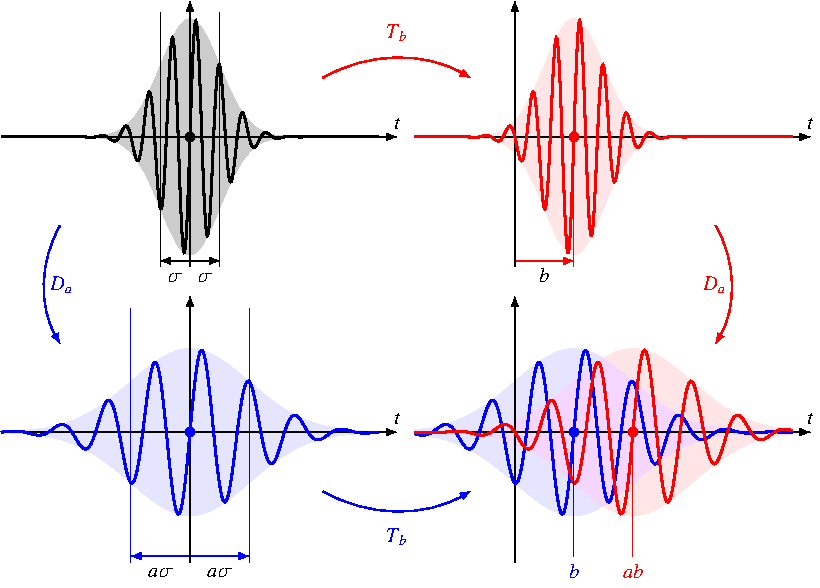
\includegraphics{chapters/2-fourier/images/kommutatorD.pdf}
\caption{Vertauschungsregel für die Operationen $T_b$ und $D_a$
(vergleiche auch Abbildung~\ref{geometrie:kommutator:image} für
die Operationen $T_b$ und $\tilde{D}_a$).
Die Graphen der Bildfunktionen unter $D_a$ sind gegenüber denen der
Bildfunktionen von $\tilde{D}_a$ vertikal um den Faktor $\sqrt{a}$
gestaucht.
\label{geometrie:kommutatorD:image}}
\end{figure}

Die Vertauschungsregel für $T_b$ und $D_a$ ist in
Abbildung~\ref{geometrie:kommutatorD:image} visualisiert.





